\documentclass[11pt, oneside]{article} 
\usepackage{geometry}
\geometry{letterpaper} 
\usepackage{graphicx}
	
\usepackage{amssymb}
\usepackage{amsmath}
\usepackage{parskip}
\usepackage{color}
\usepackage{hyperref}

\graphicspath{{/Users/telliott/Dropbox/Github-Math/geoproof/figures/}{/Users/telliott/Dropbox/Github-Math/figures/}}
% \begin{center} \includegraphics [scale=0.4] {gauss3.png} \end{center}


\title{Pythagorean theorem}
\date{}

\begin{document}
\maketitle
\Large

%[my-super-duper-separator]

We're going to develop several proofs of the Pythagorean theorem.  This theorem says that in any right triangle, the sum of the squares on the shorter sides is equal to the square on the hypotenuse.
\begin{center} 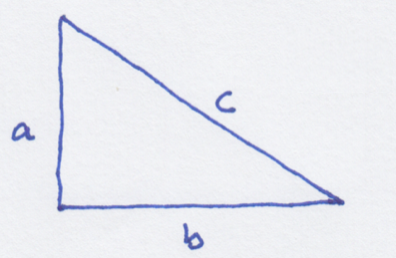
\includegraphics [scale=0.3] {E12b.png} \end{center}
\[ a^2 + b^2 = c^2 \]

The Greeks thought of it as a strictly geometric theorem, in terms of area.  We usually think of this result algebraically, for example using the integers $a = 3$, $b = 4$ and $c = 5$ to solve the equation.

Surely, first there were proofs without words.  We start with an isosceles right triangle.
\begin{center} 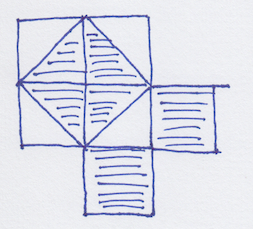
\includegraphics [scale=0.5] {J14.png} \end{center}
The square on the diagonal is obviously equal to the two small squares put together.  This is a proof of the special case of the theorem when the two small sides are equal.

But now, just tilt the inner square.
\begin{center} 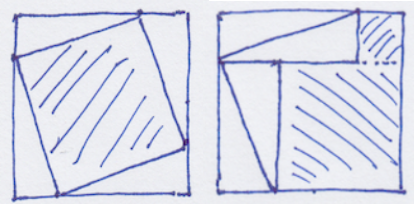
\includegraphics [scale=0.5] {J15.png} \end{center}
Four copies of the triangle take up the same space in both diagrams.  What's left is clearly the square of the hypotenuse on the left, and the sum of squares on the other sides, on the right.

\subsection*{proof from similar triangles}

We need a preliminary result.
\begin{center} 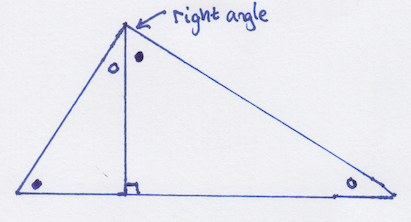
\includegraphics [scale=0.6] {J1.png} \end{center}

If we start with any right triangle, we know that the two angles which are not right angles, are complementary.  They must add up to $90$, or one right angle, by the sum of angles theorem.

So if we draw the altitude, which is perpendicular to the base and forms a right angle with it, then the two new triangles have angles that are also complementary to the originals, and therefore equal to other angles in the figure, as shown.

In the figure below, we have done the same construction.  $\angle A$ is a right angle.  The altitude or height $h$ is drawn vertically, perpendicular to the base.
\begin{center} 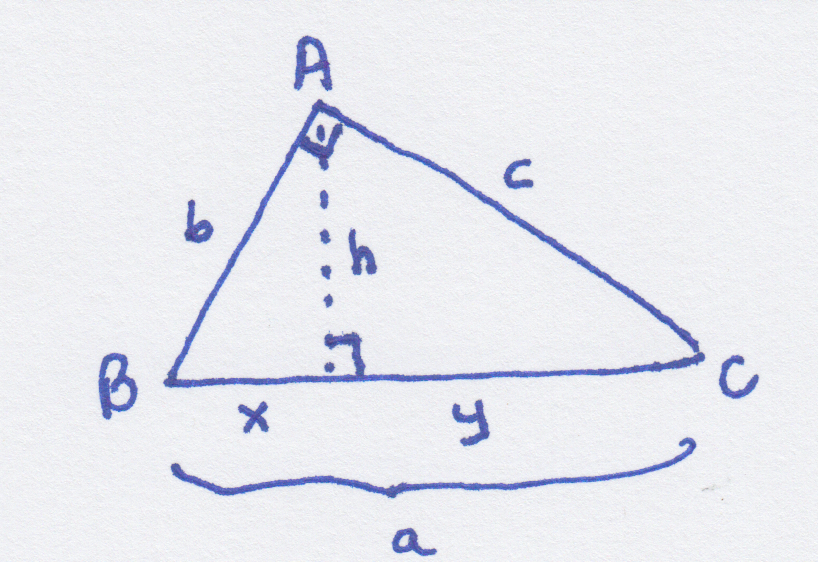
\includegraphics [scale=0.9] {J2.png} \end{center}

Our proof is a simple consequence of the relationships of similar triangles (all angles equal), namely, that corresponding sides are in the same ratio.  We postpone the demonstration of this until later, so for the moment, I hope you'll just believe me.

\emph{Proof}.

The small triangles are similar to the original.  As a result, \emph{the ratio of the hypotenuse to the short side} is equal for each, meaning that comparing the left side to the whole we get
\[ \frac{b}{x} = \frac{a}{b} \]

Similarly, the ratio of the hypotenuse to the \emph{long} side of the triangle on the right is equal to the same ratio in the original triangle:
\[ \frac{c}{y} = \frac{a}{c} \]

Rearranging, we have $b^2 = ax$ and $c^2 = ay$ so
\[ b^2 + c^2 = a(x + y) = a^2 \]

$\square$.

\subsection*{second proof}

The second proof, due to Euclid, is a little more complicated.  We need a preliminary result which we proved in the chapter on area:

\begin{center} 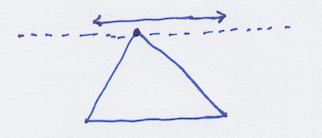
\includegraphics [scale=0.9] {E5.png} \end{center}

For any triangle, if we draw a line parallel to the base, then the apex (top vertex) can be moved anywhere along that line, and the area of the resulting triangle will be the same.

We have drawn the squares on each side of a right triangle ($\triangle DAG$).  We draw a vertical down from $D$ through 
$H$ all the way to the bottom, parallel to $AE$.
\begin{center} 
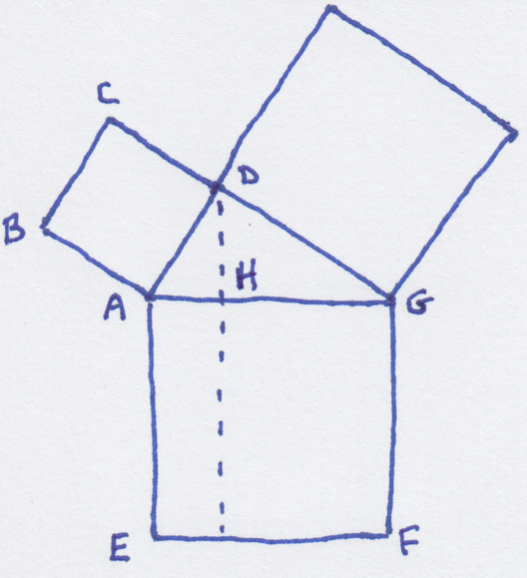
\includegraphics [scale=0.3] {J3.png} 
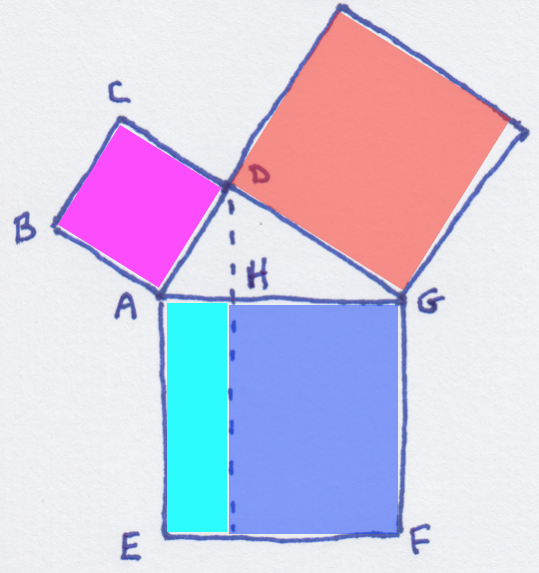
\includegraphics [scale=0.3] {J4.png} 
\end{center}
We will prove that the part of the large square that is cut off by the vertical extended from $DH$ (cyan rectangle) is equal to the entire small square (magenta).

We'll achieve that by proving that the areas of triangles formed by drawing the diagonal in each quadrilateral are equal.

\emph{To prove}.  $\triangle ABD \cong \triangle AEH$.

\begin{center} 
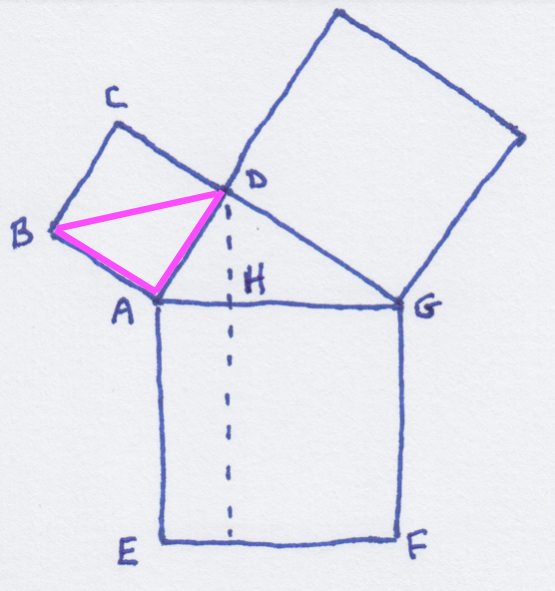
\includegraphics [scale=0.3] {J12.png} 
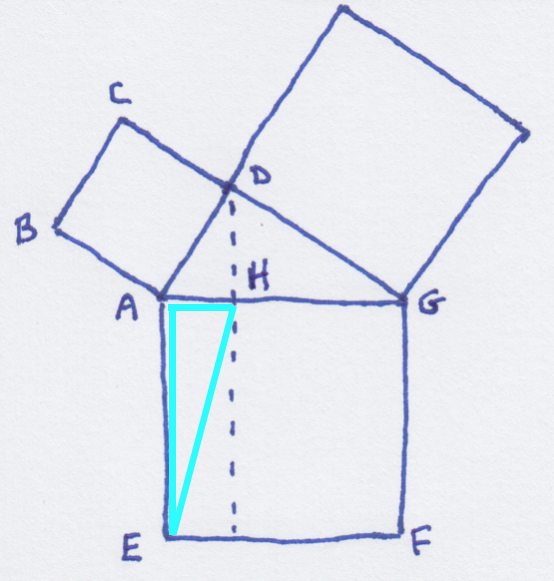
\includegraphics [scale=0.3] {J13.png} 
\end{center}

\emph{Proof}.

For the first one, compare $\triangle ABD$ and $\triangle ABG$.

\begin{center} 
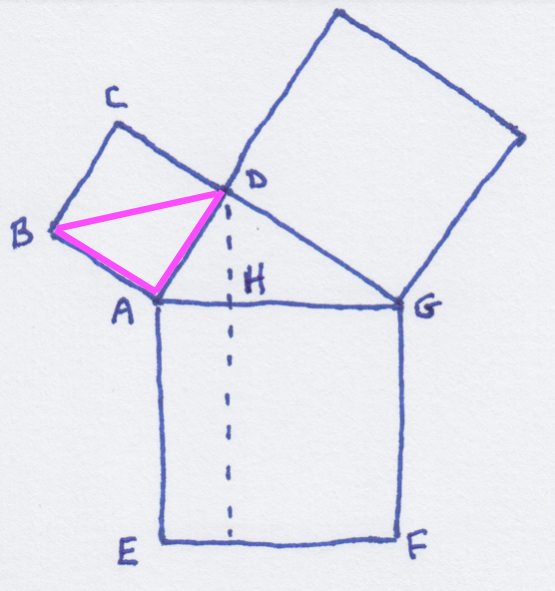
\includegraphics [scale=0.3] {J12.png} 
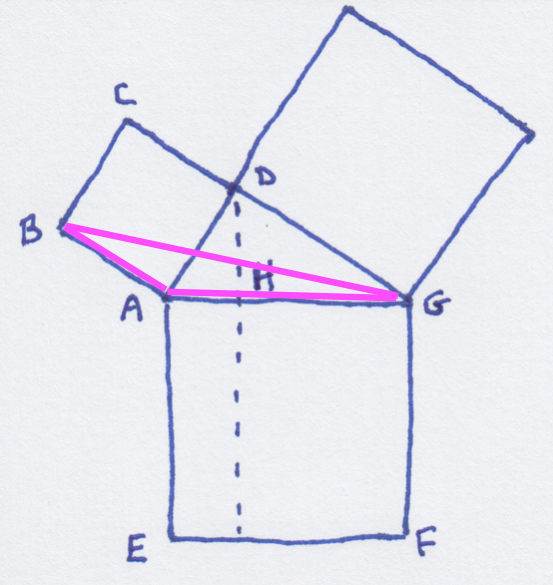
\includegraphics [scale=0.3] {J6.png} 
\end{center}

I say that the areas of the two triangles outlined in magenta are equal.  The reason is that they have the same base $AB$, and the vertex moves from $D$ to $G$ along a line $CDG$ that is parallel to the base $AB$.

\begin{center} 
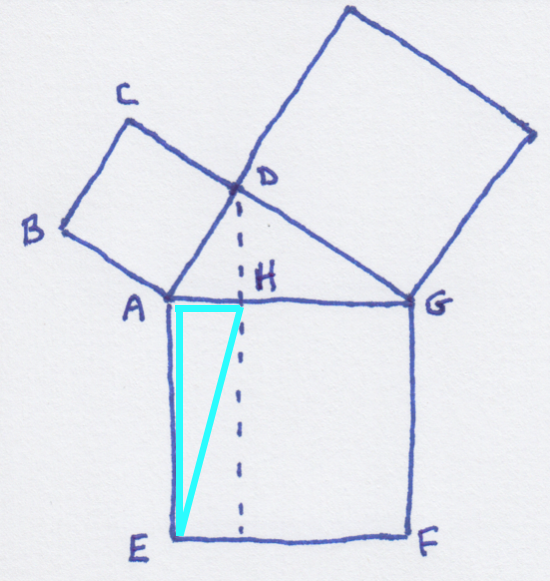
\includegraphics [scale=0.3] {J7.png} 
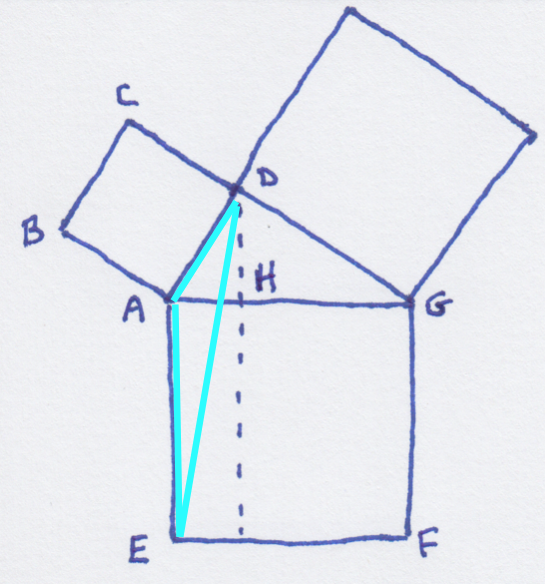
\includegraphics [scale=0.3] {J8.png} 
\end{center}

In the same way, I claim that the areas of the two triangles outlined in cyan are equal, because they have the same base $AE$ and the vertex moves from $H$ to $D$ along the line $DH$, parallel to the base $AE$.

Now we will prove that $\triangle ABG \cong \triangle ADE$.  

\begin{center} 
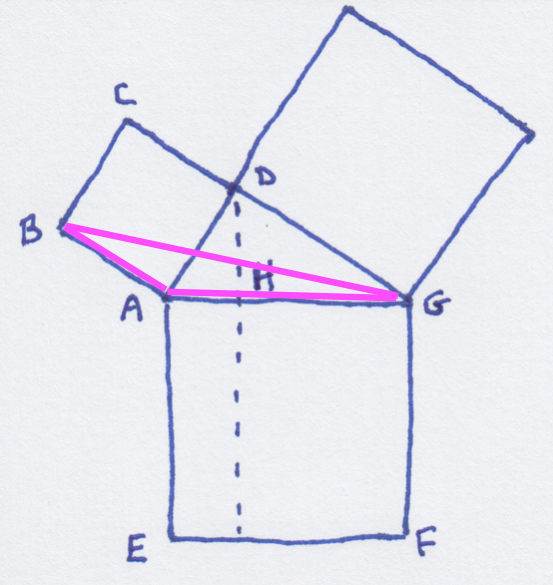
\includegraphics [scale=0.3] {J6.png} 
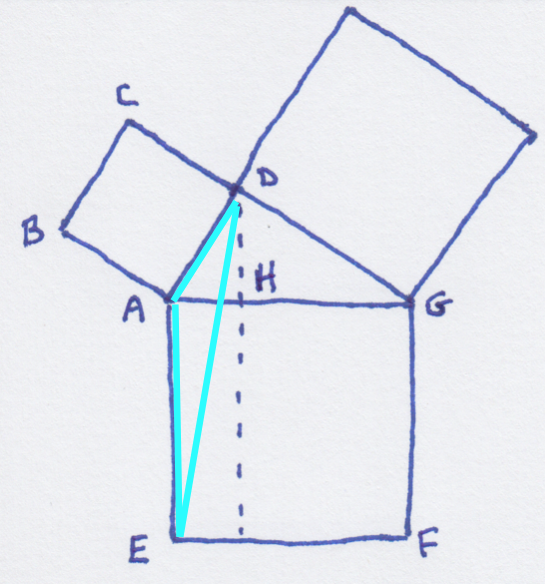
\includegraphics [scale=0.3] {J8.png} 
\end{center}

First, they share the side $AB = AD$.  They also share the side $AG = AE$.  If we can show that the central angles are equal, we will have SAS.

\begin{center} 
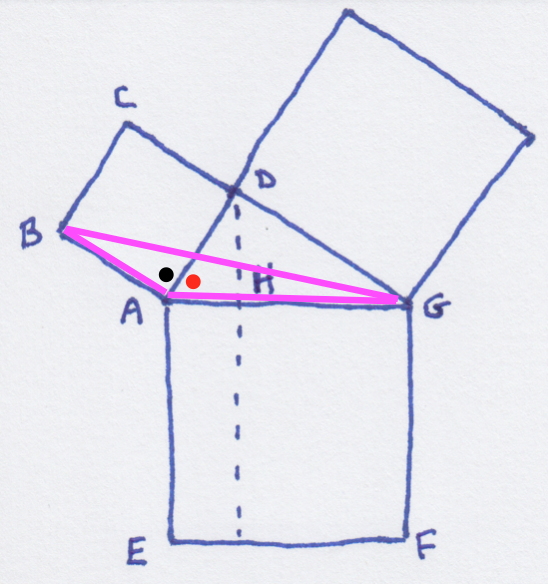
\includegraphics [scale=0.3] {J10.png} 
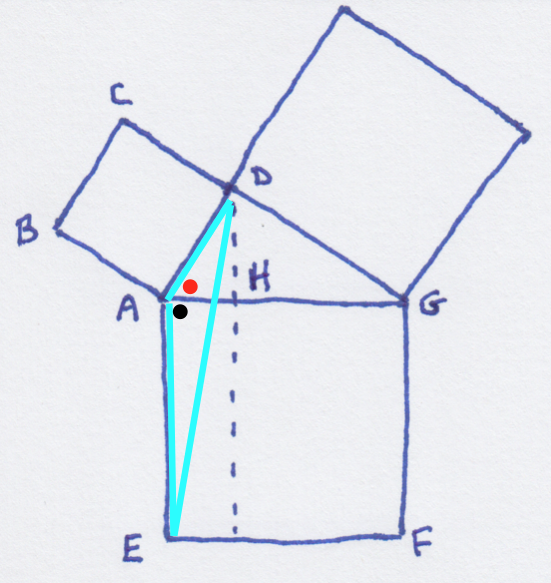
\includegraphics [scale=0.3] {J11.png} 
\end{center}

For the magenta triangle on the left, the central angle is one right angle (black dot) plus $\angle DAH$ (red dot).  

For the cyan triangle, the central angle is one right angle (black again) plus the same angle as before, $\angle DAH$.  Since each angle is the sum of a right angle and the same angle $\angle DAH$, they are equal.

\[ \angle BAG = \angle DAE \]

We have SAS.  Since each of the two triangles, $\triangle BAG$ and $\triangle ADE$, has equal area, so do the original triangles -- $\triangle BAD$ and $\triangle AEH$.

\begin{center} 
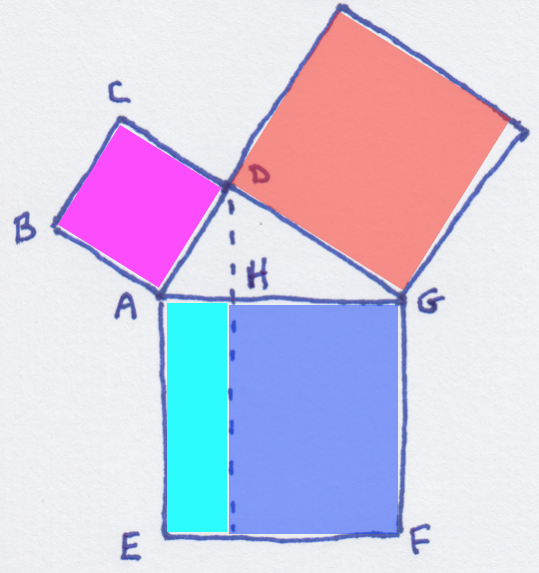
\includegraphics [scale=0.3] {J4.png} 
\end{center}

And since the magenta square and cyan rectangle are twice the triangles referenced above, they are also equal in area.  

We could repeat the argument for the other part of the figure, but we just appeal to symmetry.

$\square$.

\end{document}
